% Fig 2.2 -- nested threshold events of a cdf (web-original figure, no
%             manuscript tikzpicture; redrawn 2026-08-02 to replace the
%             hand-written SVG, which carried Chinese labels)
% Two copies of the same number line: the threshold moves from x1 to x2,
% so {X <= x1} is contained in {X <= x2}.
\documentclass[tikz,border=2pt]{standalone}
\usepackage{amsmath}
\usepackage{amssymb}
\usepackage{xcolor}
\usetikzlibrary{arrows.meta}
\newcommand{\sssig}{\scriptscriptstyle}

\definecolor{journalink}{HTML}{1F1C18}
\definecolor{journalmuted}{HTML}{8A7F72}
\definecolor{journalaccent}{HTML}{9C2D2D}

\begin{document}
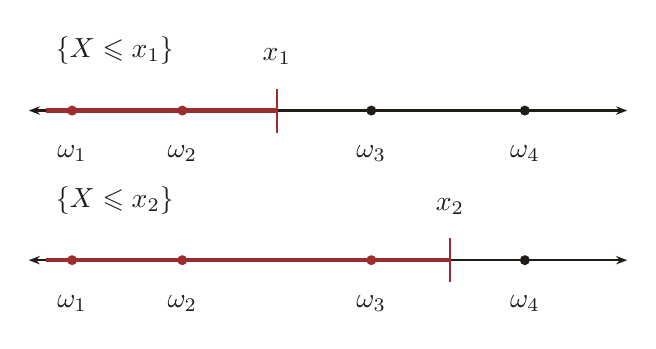
\begin{tikzpicture}[
  x=1cm,
  y=1cm,
  every node/.style={font=\normalsize, journalink},
  axis/.style={journalink, line width=0.8pt,
               {Stealth[length=4pt]}-{Stealth[length=4pt]}},
  band/.style={journalaccent, line width=1.6pt},
  thresh/.style={journalaccent, line width=0.8pt},
  solidpt/.style={circle, fill=journalink, inner sep=0pt, minimum size=3.6pt},
  accentpt/.style={circle, fill=journalaccent, inner sep=0pt,
                   minimum size=3.6pt}
]
  % ---- the two copies of the number line ----
  \draw[axis] (0,1.9) -- (7.6,1.9);
  \draw[axis] (0,0)   -- (7.6,0);

  % ---- the part of each line that the threshold takes in ----
  \draw[band] (0.22,1.9) -- (3.15,1.9);
  \draw[band] (0.22,0)   -- (5.35,0);

  % ---- threshold markers ----
  \draw[thresh] (3.15,1.62) -- (3.15,2.18);
  \draw[thresh] (5.35,-0.28) -- (5.35,0.28);

  % ---- sample points, placed at their values X(omega) ----
  \node[accentpt] at (0.55,1.9) {};
  \node[accentpt] at (1.95,1.9) {};
  \node[solidpt]  at (4.35,1.9) {};
  \node[solidpt]  at (6.30,1.9) {};

  \node[accentpt] at (0.55,0) {};
  \node[accentpt] at (1.95,0) {};
  \node[accentpt] at (4.35,0) {};
  \node[solidpt]  at (6.30,0) {};

  % ---- sample point labels ----
  \foreach \p/\k in {0.55/1, 1.95/2, 4.35/3, 6.30/4}
    \node[anchor=north] at (\p,1.58) {$\omega_{\k}$};
  \foreach \p/\k in {0.55/1, 1.95/2, 4.35/3, 6.30/4}
    \node[anchor=north] at (\p,-0.32) {$\omega_{\k}$};

  % ---- event and threshold labels ----
  \node[anchor=south west] at (0.22,2.36) {$\lbrace X\leqslant x_{1}\rbrace$};
  \node[anchor=south]      at (3.15,2.36) {$x_{1}$};
  \node[anchor=south west] at (0.22,0.46) {$\lbrace X\leqslant x_{2}\rbrace$};
  \node[anchor=south]      at (5.35,0.46) {$x_{2}$};
\end{tikzpicture}
\end{document}
